\section{Estudio de Comunidades}

\begin{figure}
    \centering  
    \begin{subfigure}[t]{0.48\textwidth}
      \centering
      \includegraphics[width=\textwidth]{img/resultados/lovaina0.5/communities-size-distribution.png}
      \caption{Coeficiente 0.5.}
    \end{subfigure}
    \vspace{7mm}
    \hfill
    \begin{subfigure}[t]{0.48\textwidth}
      \centering
      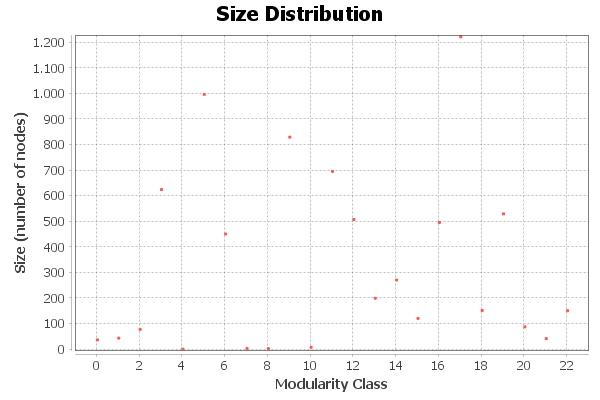
\includegraphics[width=\textwidth]{img/resultados/lovaina1/communities-size-distribution.png}
      \caption{Coeficiente 1.}
    \end{subfigure}
    \hfill
    \begin{subfigure}[t]{0.48\textwidth}
      \centering
      \includegraphics[width=\textwidth]{img/resultados/lovaina2/communities-size-distribution.png}
      \caption{Coeficiente 2.}
    \end{subfigure}
    \hfill
    \begin{subfigure}[t]{0.48\textwidth}
      \centering
      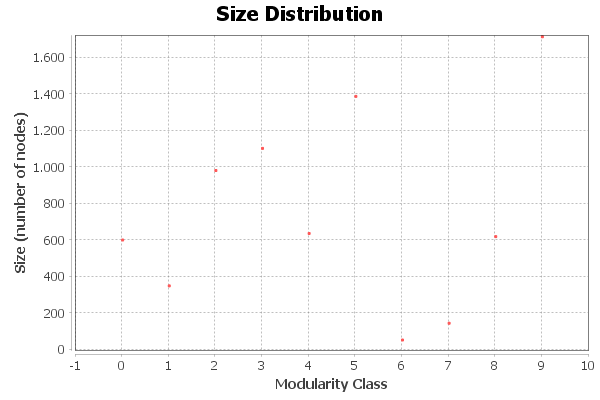
\includegraphics[width=\textwidth]{img/resultados/lovaina3/communities-size-distribution.png}
      \caption{Coeficiente 3.}
    \end{subfigure}
  
    \caption{Gráfico de distribuciones para el algoritmo Lovaina en diferentes coeficientes.}
\end{figure}

\begin{figure}
    \centering  
    \begin{subfigure}[t]{0.48\textwidth}
      \centering
      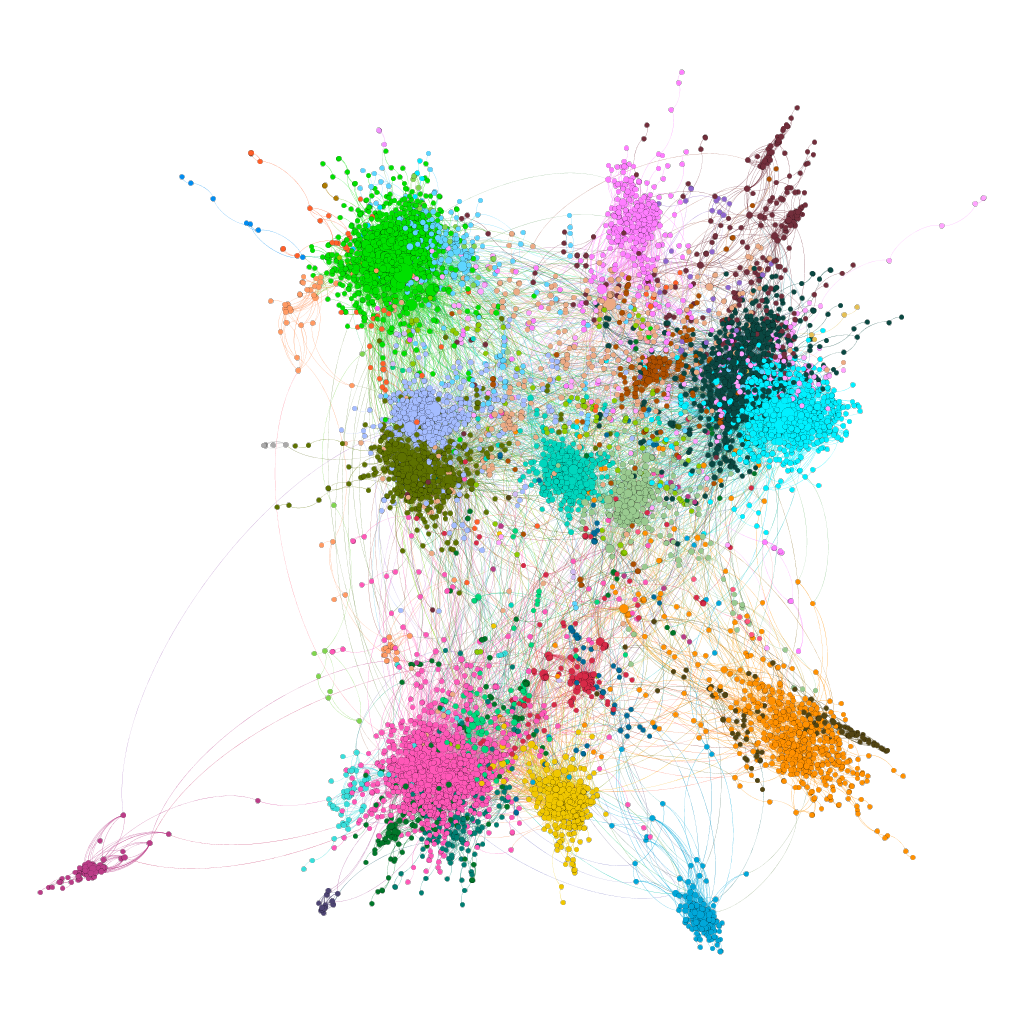
\includegraphics[width=\textwidth]{img/resultados/grado-lovaina0.5.png}
      \caption{Coeficiente 0.5.}
    \end{subfigure}
    \vspace{7mm}
    \hfill
    \begin{subfigure}[t]{0.48\textwidth}
      \centering
      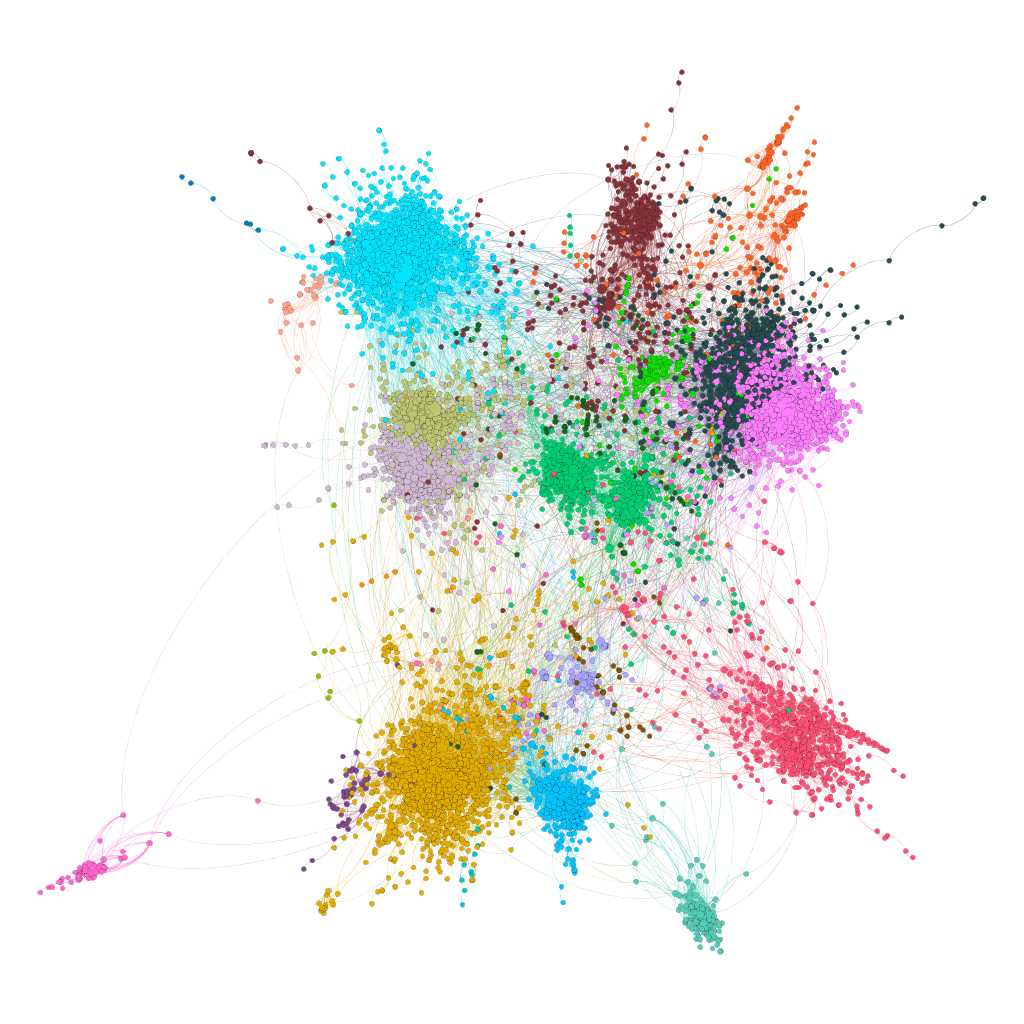
\includegraphics[width=\textwidth]{img/resultados/grado-lovaina1.png}
      \caption{Coeficiente 1.}
    \end{subfigure}
    \hfill
    \begin{subfigure}[t]{0.48\textwidth}
      \centering
      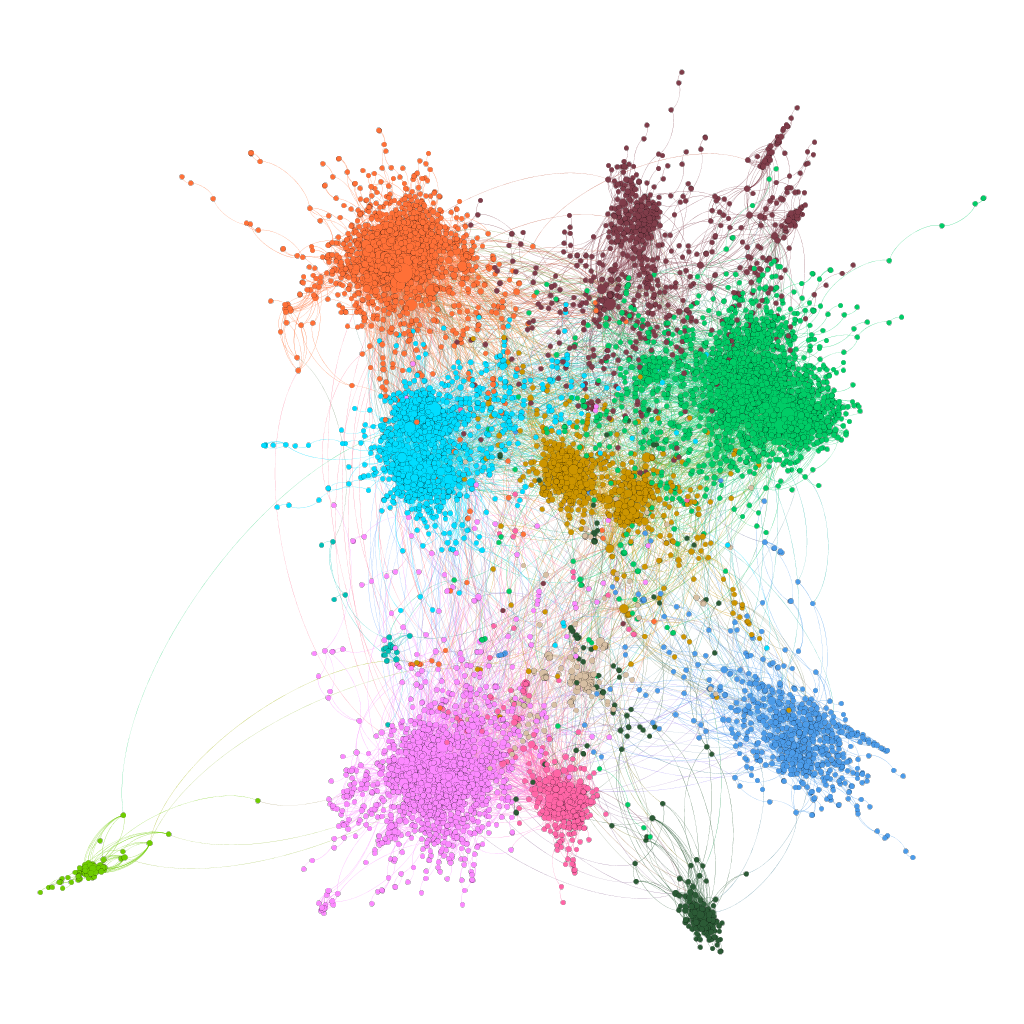
\includegraphics[width=\textwidth]{img/resultados/grado-lovaina2.png}
      \caption{Coeficiente 2.}
    \end{subfigure}
    \hfill
    \begin{subfigure}[t]{0.48\textwidth}
      \centering
      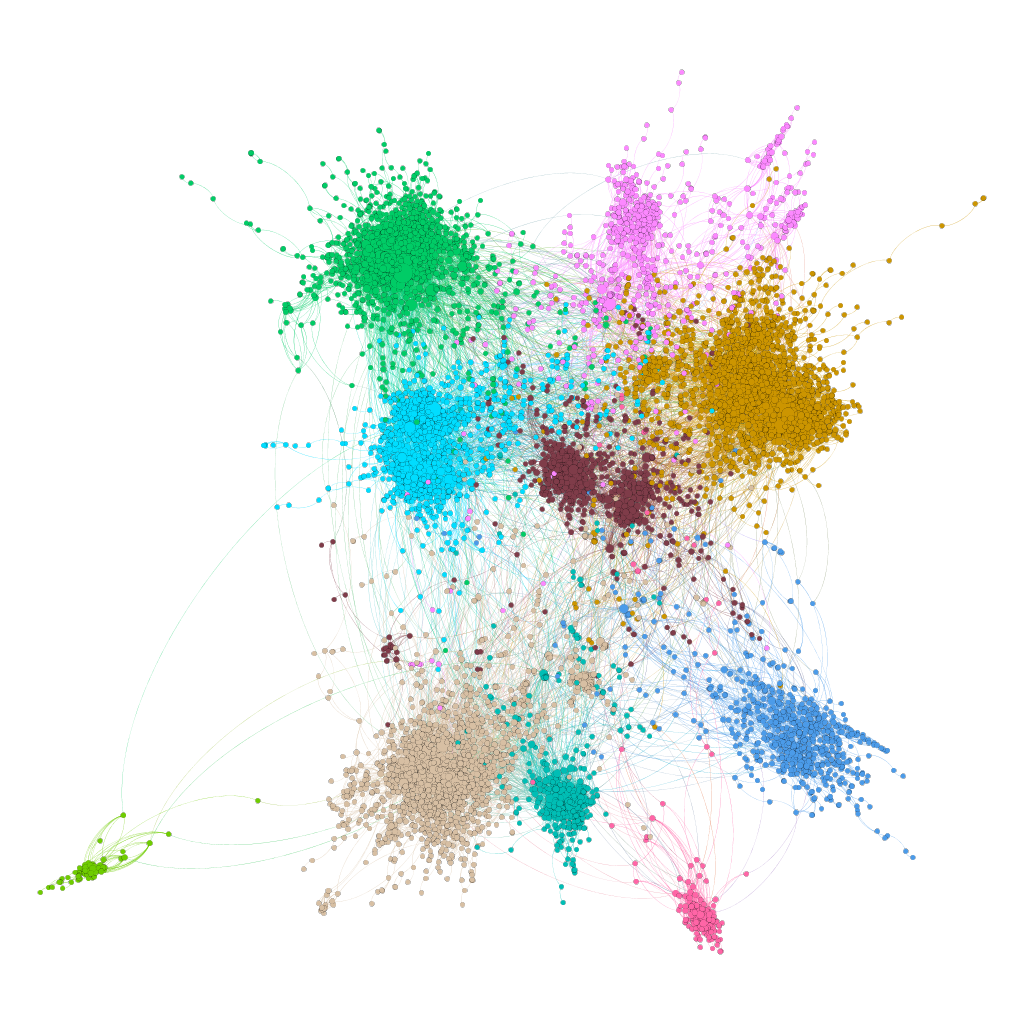
\includegraphics[width=\textwidth]{img/resultados/grado-lovaina3.png}
      \caption{Coeficiente 3.}
    \end{subfigure}
  
    \caption{Comunidades detectadas por el algoritmo Lovaina para diferentes coeficientes.}
\end{figure}

\begin{figure}
    \centering  
    \begin{subfigure}[t]{0.48\textwidth}
      \centering
      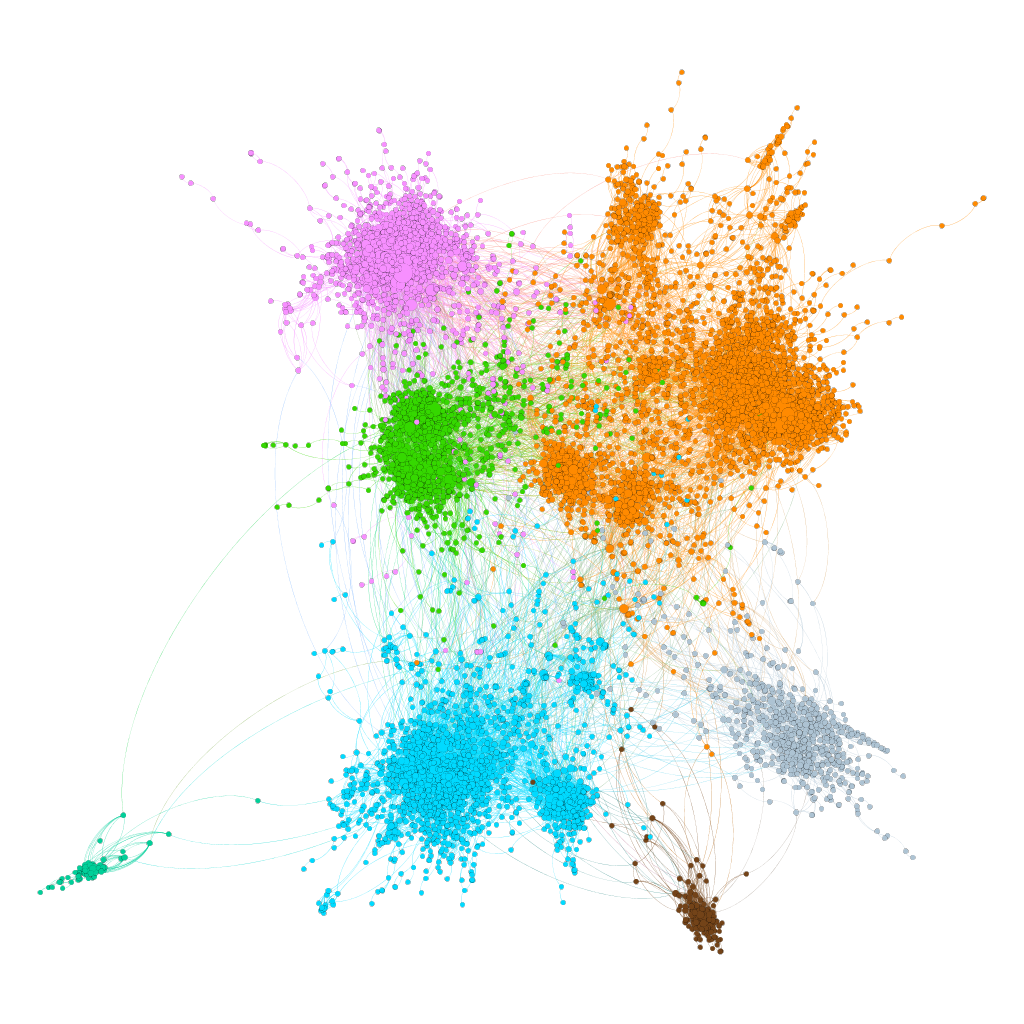
\includegraphics[width=\textwidth]{img/resultados/grado-leinen0.1.png}
      \caption{Coeficiente 0.1.}
    \end{subfigure}
    \vspace{7mm}
    \hfill
    \begin{subfigure}[t]{0.48\textwidth}
      \centering
      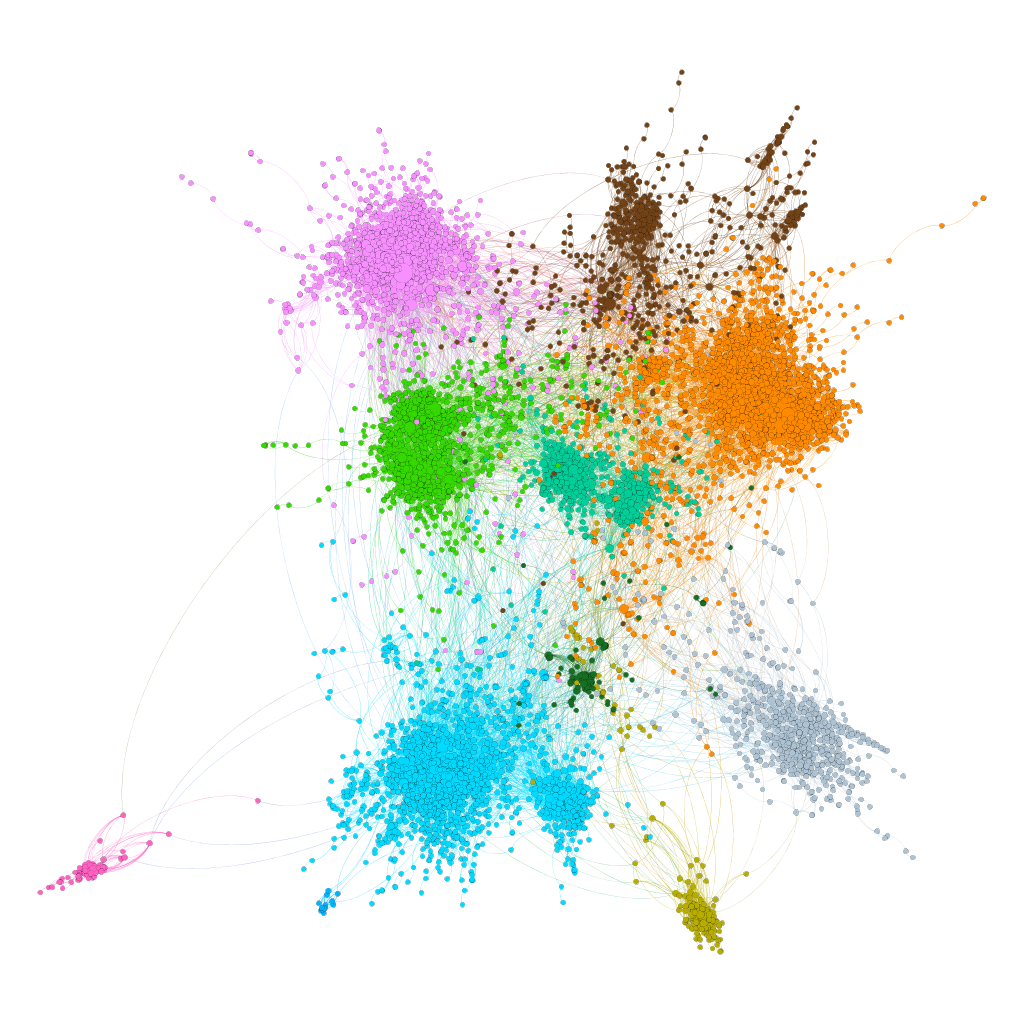
\includegraphics[width=\textwidth]{img/resultados/grado-leinen0.25.png}
      \caption{Coeficiente 0.25.}
    \end{subfigure}
    \hfill
    \begin{subfigure}[t]{0.48\textwidth}
      \centering
      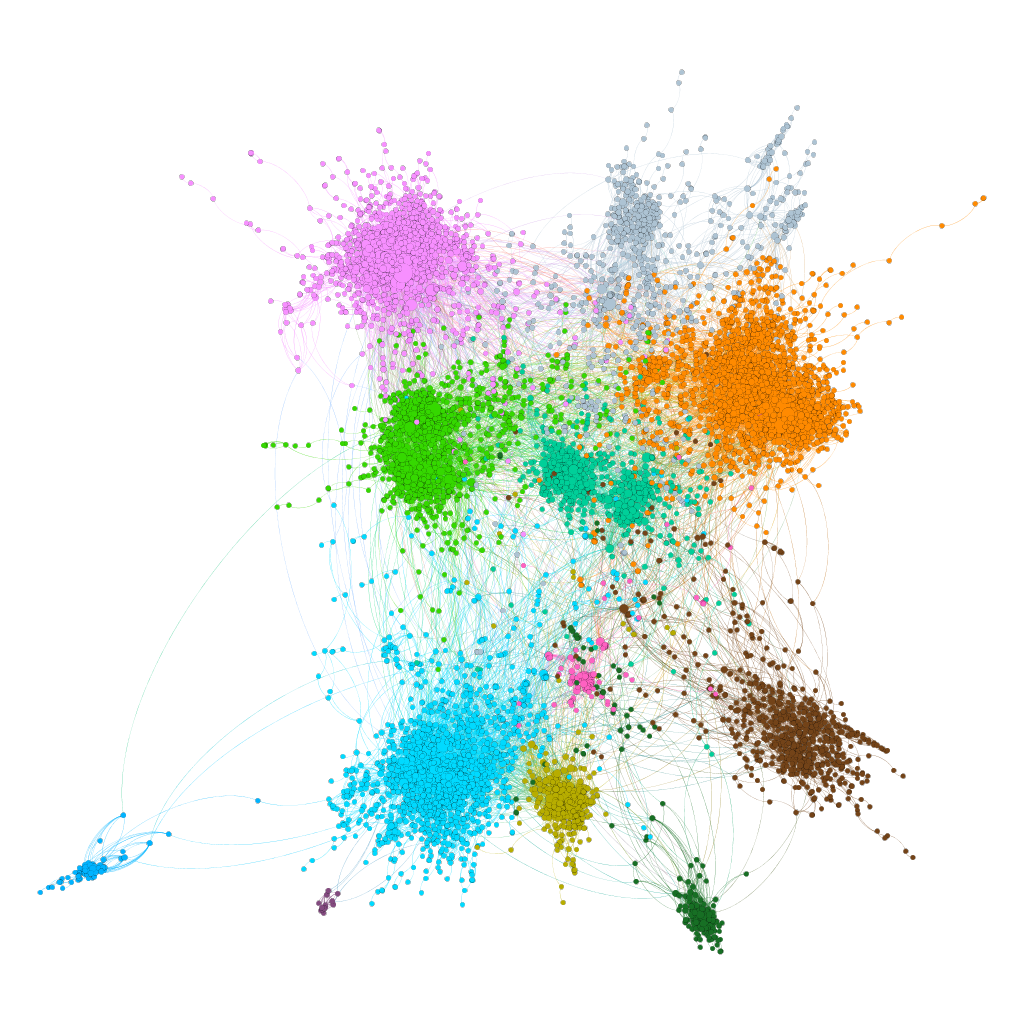
\includegraphics[width=\textwidth]{img/resultados/grado-leinen0.33.png}
      \caption{Coeficiente 0.33.}
    \end{subfigure}
    \hfill
    \begin{subfigure}[t]{0.48\textwidth}
      \centering
      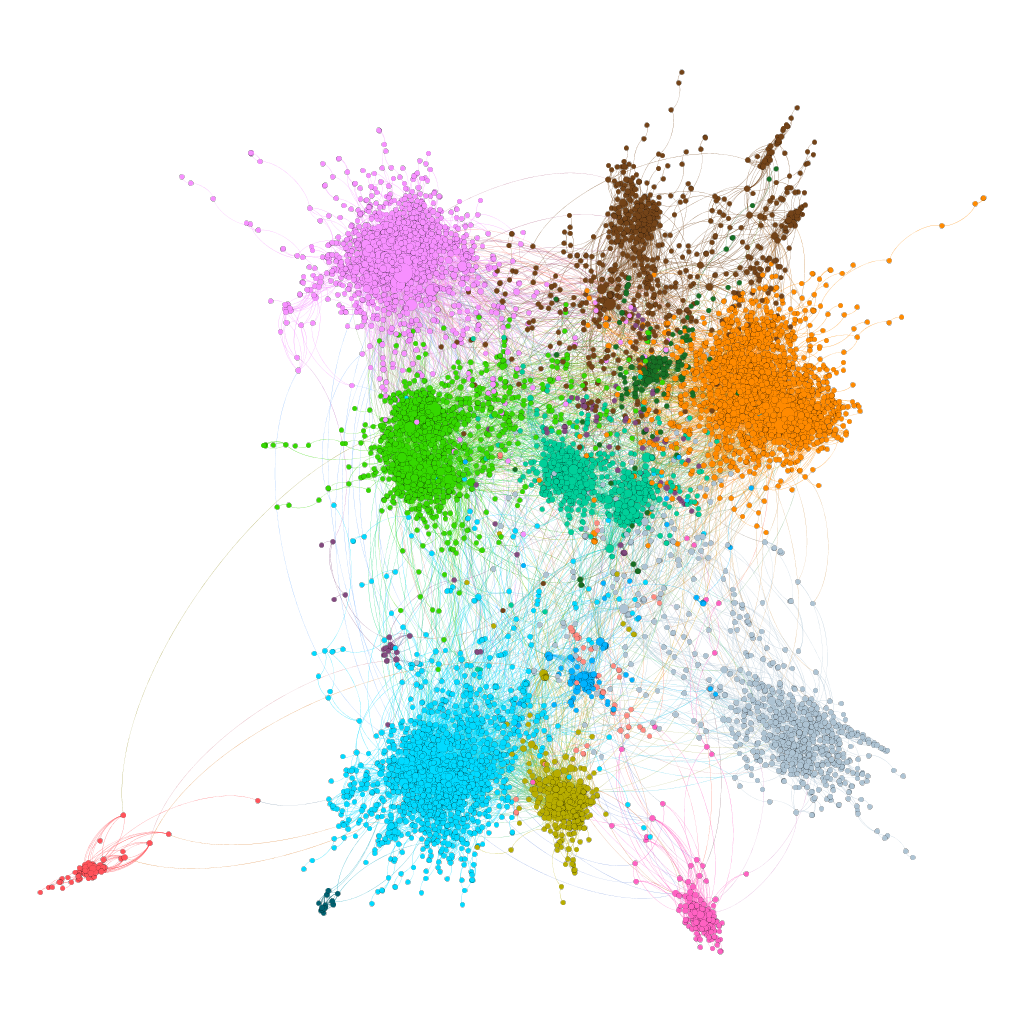
\includegraphics[width=\textwidth]{img/resultados/grado-leinen0.5.png}
      \caption{Coeficiente 0.5.}
    \end{subfigure}
  
    \caption{Comunidades detectadas por el algoritmo Leinen para diferentes coeficientes.}
\end{figure}

La referencia sobre los países puede ser un buen comienzo de partida para la búsqueda de buenas comunidades, pero es importante no dejarse engañar por eso pues por un lado existen hubs de diferentes países altamente conectados entre sí. Además, algunas de las fronteras entre los hubs de los países son difusas y existen zonas de baja conectividad fuertemente intermezcladas.

\vspace{\baselineskip}

A partir de la estructura de la red vemos que la zona central y superior del grafo no muestra una estructura modular clara. Por el contrario, la zona inferior muestra más claramente una partición en mínimo cuatro o cinco comunidades, y esto es detectado perfectamente por el método Leinen independientemente del coeficiente pero no tanto por Lovaina, donde es necesario empujar el coeficiente hacia arriba para separar mejor esto hubs.

\vspace{\baselineskip}

Resulta interesante comparar los efectos de la variación de coeficientes en ambos algoritmos.

\vspace{\baselineskip}

Sobre las comunidades en sí, visualmente concluímos que un número de diez parece adecuado para esta red, tal y como se consigue en las Figuras 16.d. De esta forma contaríamos con cinco clústers bien diferenciados en la parte inferior conectándose a un núcleo central a su vez dividido en cuatro. Este núcleo contaría con la mayoría de nodos de la red fuertemente interconectados entre sí. Por último, nos quedaría un hub denso en la parte superior izquierda con muchas conexiones al núcleo grande.

\vspace{\baselineskip}

Sobre el significado semántico de estas comunidades, es de esperar que los usuarios se agrupen por estilos y géneros de música favoritos donde el intercambio de información vaya sobre esos temas. 

De esta manera podríamos suponer que en el núcleo central predominan los géneros de moda en la cultura asiática actual (la red se construyó en 2020), como es el K-Pop, el J-Pop y el C-Pop, y que en las comunidades inferiores predominan estilos relacionados con estos géneros, pero de ámbito menos popular, como el rock, el rap, el pop anglosajón, o la música latina.

Por último, tendríamos un hub interesante en la esquina inferior izquierda, conectado al resto de la red por muy pocos nodos. En este podrían ser tendencia géneros menos relevantes como el metal, el jazz, o la electrónica.